\documentclass{article}

\title{Kolorowanie wierzchołkowe grafów}
\author{Dominik Lau}

\usepackage{blindtext}
\usepackage{amsmath}
\usepackage[utf8]{inputenc}
\usepackage[polish]{babel}
\usepackage[T1]{fontenc}
\usepackage{listings}
\usepackage{color}
\usepackage{amssymb}
\usepackage{esvect}
\usepackage{graphicx}


\graphicspath{ {./obrazy/} }

\definecolor{dkgreen}{rgb}{0,0.6,0}
\definecolor{gray}{rgb}{0.5,0.5,0.5}
\definecolor{mauve}{rgb}{0.58,0,0.82}

\lstset{frame=tb,
  language=Python,
  aboveskip=3mm,
  belowskip=3mm,
  showstringspaces=false,
  columns=flexible,
  basicstyle={\small\ttfamily},
  numbers=none,
  numberstyle=\tiny\color{gray},
  keywordstyle=\color{blue},
  commentstyle=\color{dkgreen},
  stringstyle=\color{mauve},
  breaklines=true,
  breakatwhitespace=true,
  tabsize=3
}


\begin{document}

\maketitle

\section{Definicje}

\textbf{Kolorowanie wierzchołkowe grafu} - takie przypisanie jego wierzchołkom kolorów, żeby żadne dwa sąsiednie wierzchołki nie miały tego samego koloru. \\\\
$\chi(G)$ - liczba chromatyczna grafu, ile kolorów potrzeba conajmniej, żeby go pokolorować \\\\
$D_A(n)$ - funkcja dobroci dla algorytmu A, największy stosunek wyniku algorytmu do wyniku optymalnego \\\\
$SHC(A)$ - dość trudne grafy,  grafy dla których algorytm A czasem daje wynik optymalny a czasem się myli \\\\
$HC(A)$ - trudne graf,y  grafy dla których algorytm A zawsze się myli \\\\
$\omega(G)$ - liczba klikowa grafu G, rozmiar największej kliki

\section{Oszacowania}

\subsection{Dolne}
Dla dowolnego grafu o $\omega(G) = \omega$ mamy$ \chi(G) \ge \omega $. \\
Różnica może być dowolnie duża,  np. grafy Mycielskiego

\begin{center}
\includegraphics[width=5cm]{Mycielski}
\end{center}

\subsection{Górne}
Dla dowolnego grafu o $\Delta(G) = \Delta$ mamy $\chi(G) \leq \Delta + 1$.  \\
\textbf{Tw. Brooksa}: $\chi(G) = \Delta + 1$ tylko dla grafów pełnych i cykli nieparzystych. \\\\
Dla grafów planarnych mamy $\chi(G) \leq 4$.


\section{Funkcja dobroci}

\begin{gather*}
	D_A(n) =\underset{G, |V(G)| = n}{max} \frac{A(G)}{OPT(G)} \\
\end{gather*} 
W kolorowaniu najlepszą funkcją jest $D_A(n) = 1$, najgorszą $D_A(n) = n$ (bo taki wynik daje algorytm trywialny kolorujący wszystkie wierzchołki na różne kolory).


\section{SL - smallest last}

\subsection{Działanie algorytmu}
Złożoność -  $O(n+m)$ \\\\
Pseudokod
\begin{lstlisting}
def SL(G):
	G2 = copy(G)
	kolejnosc = []
	while n(G2) != 0:
		v = wierzcholek_o_min_deg(G2)
		kolejnosc.push_front(v)
		G2 = G2 - v

	pokoloruj_zachlannie(G,kolejnosc)
		
\end{lstlisting}

\subsection{Przypadki pozytywne}

SL optymalnie koloruje drzewa, ponieważ zostawia liście na koniec. \\\\
inne optymalne: drzewa, cykle \\
półpozytywne (funkcja dobroci O(1)): grafy Johnsona, grafy Mycielskiego, grafy planarne

\subsection{Trudne grafy}
$min(SHC(A)) = $ PRYZMA 
\begin{center}
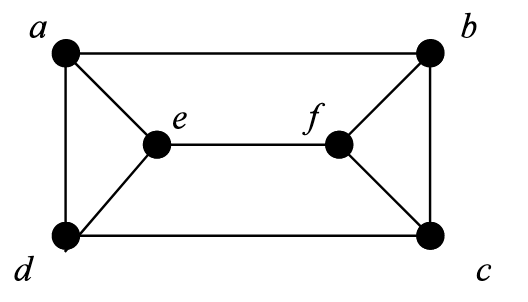
\includegraphics[width=5cm]{pryzma}
\end{center}
$min(HC(A)) = $ PRYZMOID
\begin{center}
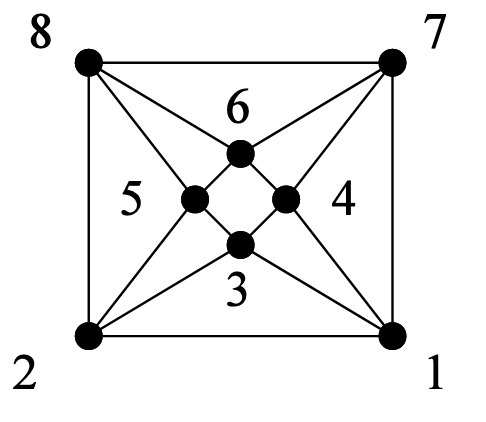
\includegraphics[width=5cm]{pryzmoid}
\end{center}
\subsection{Funkcja dobroci}
Dla grafu Colmena Moora $CM_k$ (poniżej $CM_3$)
\begin{center}
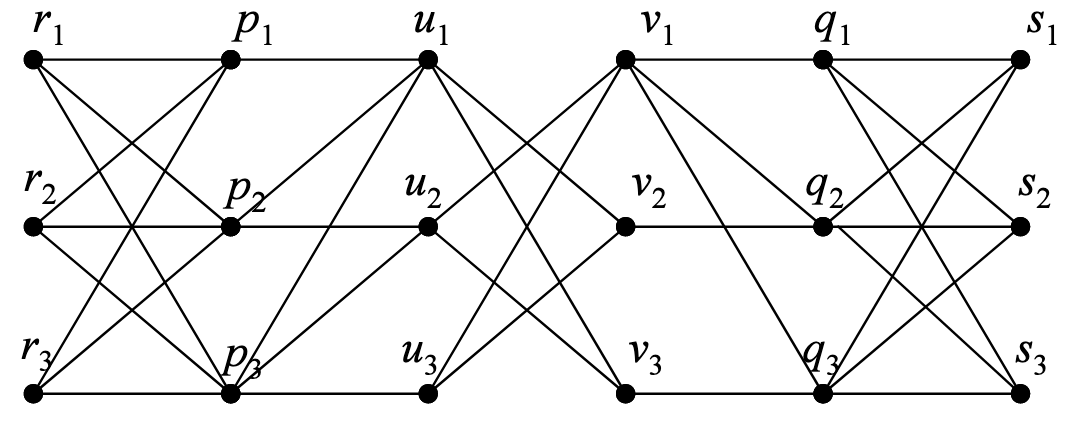
\includegraphics[width=5cm]{CM}
\end{center}
SL użyje k-kolorów (k $\sim$ n) mimo, że jest to graf dwudzielny $\rightarrow D_{SL}(n) = O(n)$

\section{LF - largest first}
\subsection{Działanie algorytmu}
Złożoność - $O(n+m)$ \\\\
Pseudokod
\begin{lstlisting}
def LF(G):
	kolejnosc = wierzcholki_od_max_deg_do_min_deg(G)
	pokoloruj_zachlannie(G,kolejnosc)
\end{lstlisting}

\subsection{Trudne/dość trudne grafy}
 $min (SHC(A)) = P_6$ 
\begin{center}
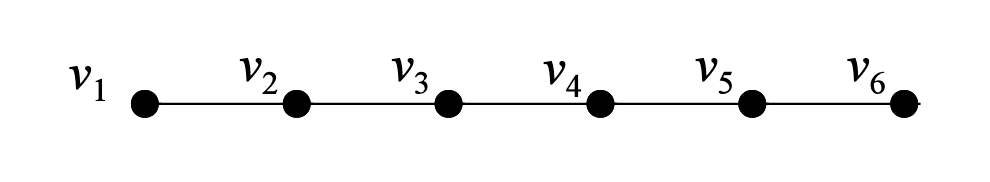
\includegraphics[width=10cm]{P6}
\end{center}
 $min (HC(A)) = $KOPERTA
\begin{center}
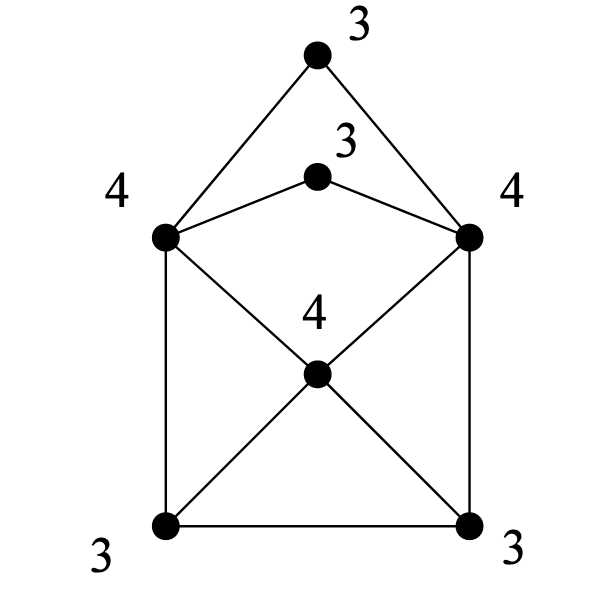
\includegraphics[width=5cm]{Koperta}
\end{center}

\subsection{Funkcja dobroci}
Najgorszy przypadek zachodzi dla grafów Jordana $J_k$.  Poniżej $J_4$ .
\begin{center}
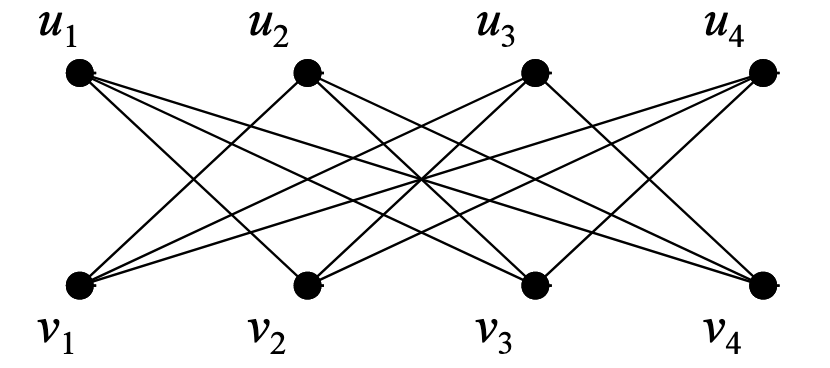
\includegraphics[width=5cm]{Jordan}
\end{center}
LF pokoloruje je $k = \frac{n}{2}$ kolorami $\rightarrow$ $D_{LF}(n) = n/4 = O(n)$.

\section{Grafy planarne}
Algorytm SL koloruje grafy planarne co najwyżej 6 kolorami. Z czego to wynika?

\section{Inne}
\textbf{W ogólności oba algorytmy nie kolorują optymalnie grafów dwudzielnych. }\\\\
Graf "jajca"
\begin{center}
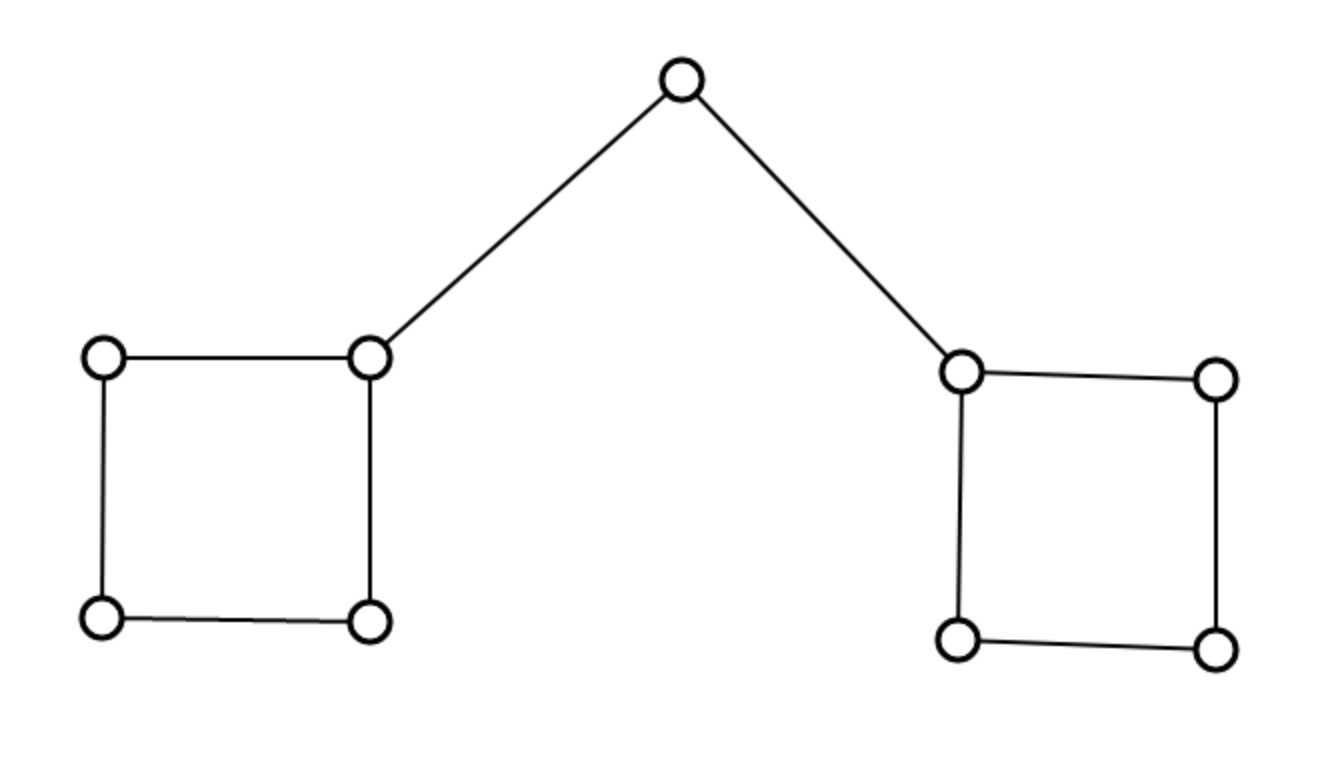
\includegraphics[width = 5cm]{jajco}
\end{center}
Jest to graf dwudzielny,  dość trudny dla SL (może mylić się o 1), który LF koloruje optymalnie. \\\\
Graf "poczwórne jajca"
\begin{center}
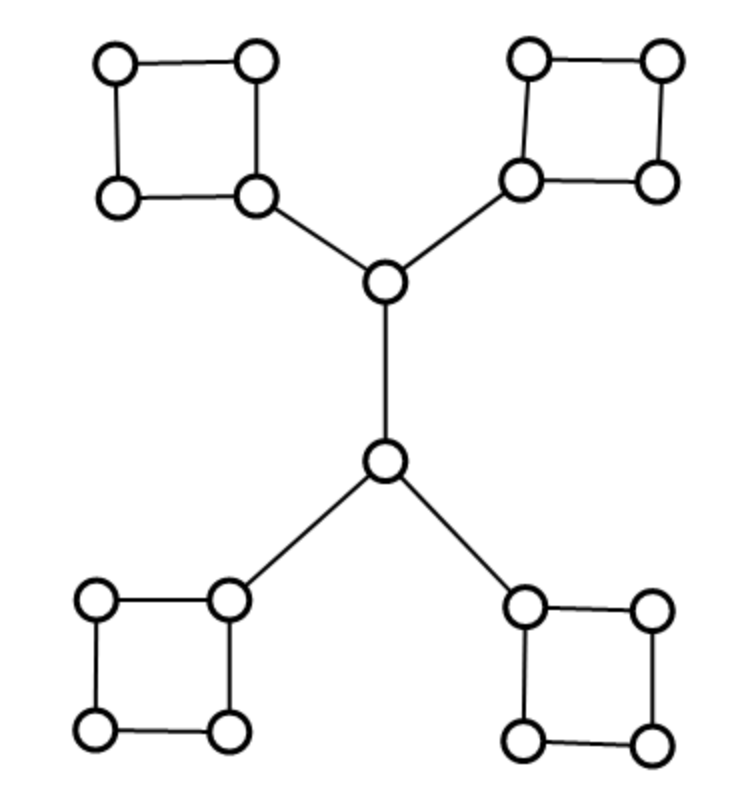
\includegraphics[width=5cm]{czteryjaja}
\end{center}
Jest to graf dwudzielny, dość trudny dla SL (może się mylić o 2), który LF koloruje optymalnie. \\\\


\end{document}
